% !TeX spellcheck = en_US
% !TeX encoding = UTF-8
\documentclass[11pt, a4paper, final]{amsart}
\setlength{\emergencystretch}{2em}


\usepackage[T1]{fontenc}
\usepackage{lmodern}
\usepackage{mathtools}
%\usepackage[activate={true,nocompatibility},final,tracking=true,kerning=true,spacing=true,stretch=10,shrink=10]{microtype}
%\microtypecontext{spacing=nonfrench}
\usepackage[utf8]{inputenc}

\topmargin0pt
\oddsidemargin0pt
\evensidemargin0pt
\textheight660pt
\textwidth445pt

\usepackage{amsfonts}
\usepackage{amsmath}
\usepackage{amssymb}
\usepackage{amsthm}
\usepackage{mathtools}
\usepackage{paralist, tabularx}
\usepackage{enumitem}
\usepackage[utf8]{inputenc}
\usepackage{mathabx,epsfig}
\usepackage{tikz-cd}
\usepackage{verbatim}


\usepackage{etoolbox}


\usepackage{xcolor}
\definecolor{green}{RGB}{0,127,0}
\definecolor{redd}{RGB}{191,0,0}
\definecolor{red}{RGB}{105,89,205}
\usepackage[colorlinks=true]{hyperref}

\usepackage[notref, notcite]{showkeys}
\usepackage[cmtip,arrow]{xy}

%%%%%%%%%%%%%%%%%%%%%%%%%%%%%%%%%%%%%%%%%%%%%%%%%%%%%%%%%%%%%%%%
\begin{comment}
\usepackage[backend=biber,
url=false,
isbn=false,
backref=true,
citestyle=alphabetic,
bibstyle=alphabetic,
autocite=inline,
maxnames=99,
minalphanames=4,
maxalphanames=4,
sorting=nyt,]{biblatex}
\addbibresource{two_three_steps.bib}
\end{comment}

\usepackage{filecontents}
\begin{filecontents}{references.bib}

\end{filecontents}

\usepackage[
backend=bibtex,
%style=alphabetic,
url=false,
isbn=false,
backref=true,
citestyle=alphabetic,
bibstyle=alphabetic,
autocite=inline,
maxnames=99,
minalphanames=4,
maxalphanames=4,
sorting=nyt,
]{biblatex}

\addbibresource{references.bib}
%%%%%%%%%%%%%%%%%%%%%%%%%%%%%%%%%%%%%%%%%%%%%%%%%%%%%%%%%%%%%%%%


\DeclareMathOperator{\Aut}{Aut}
\DeclareMathOperator{\Sym}{Sym}
\DeclareMathOperator{\Hom}{Hom}
\DeclareMathOperator{\UT}{UT}
\DeclareMathOperator{\T}{T}
\DeclareMathOperator{\Stab}{Stab}
\DeclareMathOperator{\st}{st}
\newcommand{\Bohr}[1]{{#1}^{\textrm{Bohr}}}
\newcommand{\R}{{\mathbb{R}}}
\newcommand{\Z}{{\mathbb{Z}}}
\newcommand{\N}{{\mathbb{N}}}
\newcommand{\ZZ}{{\bar{\Z}}}
\newcommand{\G}{{\bar{G}}}
%\newcommand{\M}{{\bar{M}}}
\newcommand{\RR}{{\bar{R}}}
\newcommand{\Lset}{\mathcal{L}_{set}}
\newcommand{\Lsetp}[1]{\mathcal{L}_{set,{#1}}}
\newcommand{\LL}{\mathcal{L}}
\newcommand{\FF}[1]{\mathbb{F}_{#1}}
\DeclareMathOperator{\error}{{error}}
\DeclareMathOperator{\Mor}{Mor}
\DeclareMathOperator{\ext}{ext}
\DeclareMathOperator{\id}{id}

\newcommand{\Ra}{(R,+)}
\newcommand{\RRa}{(\RR,+)}
\newcommand{\RRaD}{(\RR,+)^{0}}
\newcommand{\RRaT}{(\RR,+)^{00}}
\newcommand{\RRaI}{(\RR,+)^{000}}
\newcommand{\RRiD}{\RR^{0}}
\newcommand{\RRiT}{\RR^{00}}
\newcommand{\RRiI}{\RR^{000}}

\newcommand{\C}{\mathfrak{C}}
\newcommand{\M}{{\mathcal M}}



\newcommand{\Za}{(\Z,+)}
\newcommand{\ZZa}{(\ZZ,+)}
\newcommand{\ZZaD}{(\ZZ,+)^{0}}
\newcommand{\ZZaT}{(\ZZ,+)^{00}}
\newcommand{\ZZiD}{\ZZ^{0}}
\newcommand{\ZZiT}{\ZZ^{00}}



\newcommand\todo[1]{\textbf{\textcolor{redd}{#1}}}


\newcommand{\nref}[2]{\hyperref[#1]{\ref*{#1}$_{#2}$}}

\newcommand{\cupdot}{\mathbin{\mathaccent\cdot\cup}}


\DeclareMathOperator{\topo}{{top}}
\DeclareMathOperator{\im}{{Im}}
\DeclareMathOperator{\lin}{{Lin}}
\DeclareMathOperator{\Th}{{Th}}
\DeclareMathOperator{\SL}{{SL}}
\DeclareMathOperator{\tp}{{tp}}
\DeclareMathOperator{\cl}{{cl}}
\DeclareMathOperator{\dcl}{{dcl}}

%%%%%%%%%%%%%%%%%%%%%%%%%%%%%%%%%%%%%%%%%%%%%%%%%%%%%%%%%%%% NASZE KOMENDY %%%%%%%%%%%%%%%%%%%%%%%%%%

\newcommand{\sphere}{\mathcal{S}}
\newcommand{\disk}{\mathcal{D}}
\newcommand{\pt}{\star}

\DeclareMathOperator{\SO}{SO}
\DeclareMathOperator{\Ext}{Ext}
\DeclareMathOperator{\Tor}{Tor}

%%%%%%%%%%%%%%%%%%%%%%%%%%%%%%%%%%%%%%%%%%%%%%%%%%%%%%%%%%%%%%%%%%%%%%%%%%%%%%%%%%%%%%%%%%%%%%%%%%%%%


\newtheorem{theorem}{Theorem}
\numberwithin{theorem}{section}
\newtheorem{lemma}[theorem]{Lemma}
\newtheorem{claim}[theorem]{Claim}
\newtheorem{fact}[theorem]{Fact}
\newtheorem{proposition}[theorem]{Proposition}
\newtheorem{problem}[theorem]{Problem}
\newtheorem{conjecture}[theorem]{Conjecture}
\newtheorem{axiom}[theorem]{Axiom}
\newtheorem{question}[theorem]{Question}
\newtheorem{corollary}[theorem]{Corollary}
\newtheorem*{theorem2}{Theorem}
\newtheorem*{claim2}{Claim}
\newtheorem*{corollary2}{Corollary}
\newtheorem*{question2}{Question}
\newtheorem*{conjecture2}{Conjecture}


\newtheorem{clm}{Claim}
\newtheorem*{clm*}{Claim}


\theoremstyle{definition}
\newtheorem{definition}[theorem]{Definition}
\newtheorem*{definition2}{Definition}
\newtheorem{example}[theorem]{Example}

\theoremstyle{remark}
\newtheorem{remark}[theorem]{Remark}
\newtheorem*{remark2}{Remark}


\AtEndEnvironment{proof}{\setcounter{clm}{0}}
\newenvironment{clmproof}[1][\proofname]{\proof[#1]\renewcommand{\qedsymbol}{$\square$(claim)}}{\endproof}

\usepackage[hyphenbreaks]{breakurl}

%\usepackage{filecontents}
%\begin{filecontents}{references.bib}

%\end{filecontents}

\usepackage[
backend=bibtex,
%style=alphabetic,
url=false,
isbn=false,
backref=true,
citestyle=alphabetic,
bibstyle=alphabetic,
autocite=inline,
maxnames=99,
minalphanames=4,
maxalphanames=4,
sorting=nyt,
]{biblatex}

\usepackage{calligra}


%\addbibresource{references.bib}

\title{Hatcher solutions}

\author{Michał Mądrala}
\author{Ruba Rudzik}
\author{Krzysztof Szymański}

\begin{document}

	\begin{abstract}
	       We present the solutions to the excercises found in Allen Hatcher's ,,Algebraic Topology'' \cite{AH} with our own perspective and commentary. We also present proofs of selected theorems (with what we hope is a more detailed explanation). 
	\end{abstract}
	
\maketitle

\begin{center}
    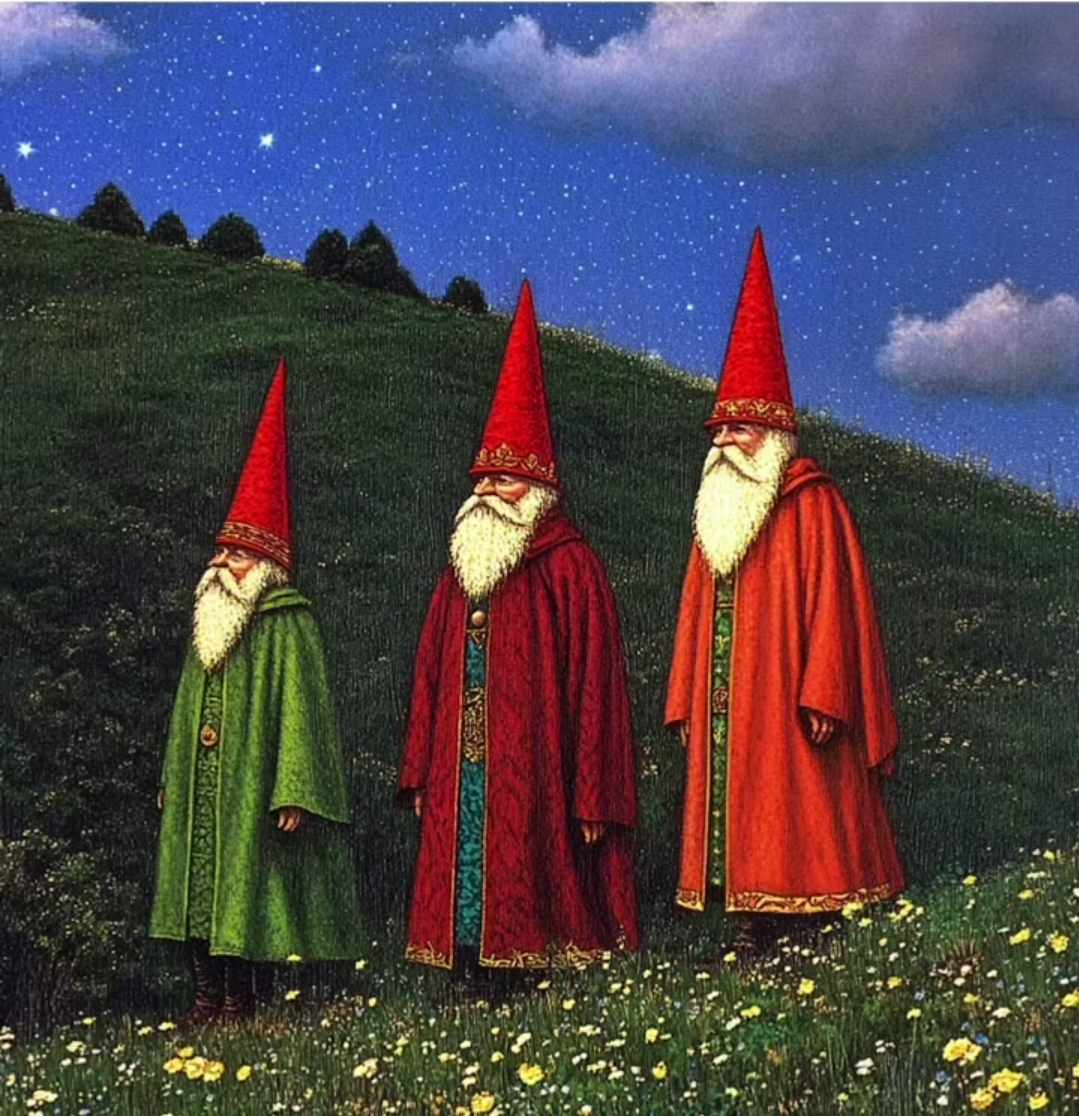
\includegraphics[width=120mm]{jd_śwg_jśw.jpg}
\end{center}

\begin{center}
    {\fontfamily{pzc}\selectfont Dedicated to Jan Dymara, Światosław Gal \& Jacek Świątkowski}
    %{\calligra Dedicated to Jan Dymara, Swiatoslaw Gal, Jacek Świątkowski}
\end{center} 

\newpage

\section{The Fundamental Group}

\subsection{Basic Constructions}

This section is about basic constructions.

\todo{Należałoby poprawić numerację problemów, żeby była tak jak w hatcherze, no i też żeby sekcje w Additional Topics nie były 2.4 itp tylko 2.A, 2.B itd}

\begin{problem}\label{problem: 1.1.1}
Show that composition of paths satisfies the following cancellation property: If
$f_0 \cdot g_0 \simeq f_1 \cdot g_1$ and $g_0 \simeq g_1$ then $f_0 \simeq f_1$.
\end{problem}

\begin{proof}
    
\end{proof}

\begin{problem}\label{problem: 1.1.9}
    Let $A_1 , A_2 , A_3$ be compact sets in $\R^3$ . Use the \textbf{Borsuk–Ulam theorem} to show
that there is one plane $P \subseteq \R^3$ that simultaneously divides each $A_i$ into two pieces of
equal measure.
\end{problem}

Let us introduce some notation. Let $\lambda$ denote the measure we are interested in. We can think of the set of all planes in $\R^3$, as $\sphere^2\times\R$, thus for a plane $P$, let $P_{n, t}$ denote the plane with a normal vector $n \in \mathcal{S}^2$, moved along it by $t \in \R$. We denote by $P^+_{n, t}, P^-_{n, t}$ two halves of $\R^3$, respectively above and below the $P_{n, t}$ (in the sense of direction of $n$). We will need the following lemma:

\begin{lemma}\label{lemma: about continous equal-cutting}
    Let $A \subseteq \R^3$ be a compact subset, there exists a continous, \textbf{even} map $h : \sphere^2 \xrightarrow{} \R$, such that:
    $$\lambda(P^+_{n, h(n)} \cap A) = \lambda(P^-_{n, h(n)} \cap A)$$
\end{lemma}

The idea behind the lemma is to find a continous family of planes, each equally dividing given set.
\todo{Zauważyliśmy, że potrzeba żeby ta mapa była parzysta.}

\begin{proof}\textit{(of the Lemma \ref{lemma: about continous equal-cutting})}
    \todo{TODO}
\end{proof}

\begin{proof}\todo{utworzyć begin-solution i tutaj zmienić)}
    Construct $h : \sphere^2 \to \R$ as in Lemma \ref{lemma: about continous equal-cutting} for $A_1$.
    Let $g : \sphere^2 \to \R^2$ be defined as follows:
    \[\begin{tikzcd}
	{\sphere^2} && {\R^2} \\
	n && {\begin{pmatrix}
	    \lambda(P^+_{n, h(n)} \cap A_2) \\
        \lambda(P^+_{n, h(n)} \cap A_3)
	\end{pmatrix}}
	\arrow["g", from=1-1, to=1-3]
	\arrow["\in"{marking, allow upside down}, draw=none, from=2-1, to=1-1]
	\arrow[maps to, from=2-1, to=2-3]
	\arrow["\in"{marking, allow upside down}, draw=none, from=2-3, to=1-3]
\end{tikzcd}\]
\todo{Ten diagram to tylko fleks z użycia quivera, można to napisać normalnie i pewnie będzie ładniej.} \\
Since $h$ is continous, $g$ is continous as well. By the \textbf{Borsuk-Ulam theorem}, there exists some $n \in \sphere^2$, such that:
$$\begin{pmatrix}
	    \lambda(P^+_{n, h(n)} \cap A_2) \\
        \lambda(P^+_{n, h(n)} \cap A_3)
	\end{pmatrix} = \begin{pmatrix}
	    \lambda(P^+_{-n, h(-n)} \cap A_2) \\
        \lambda(P^+_{-n, h(-n)} \cap A_3)
	\end{pmatrix} = \begin{pmatrix}
	    \lambda(P^-_{n, h(n)} \cap A_2) \\
        \lambda(P^-_{n, h(n)} \cap A_3)
	\end{pmatrix}$$
    The last equality follows from evenness of $h$, and the fact that $P^+_{-n, t} = P^-_{n, t}$.
    \todo{Zamiast tych pmatrixów można pisać $A_i$}
\end{proof}

\begin{problem}\label{problem: 1.1.18}
    
\end{problem}

\subsection{Van Kampen's Theorem}
\subsection{Covering Spaces}
\subsection{Additional Topics}
\subsubsection{Graphs and Free Groups}
\subsubsection{$\mathcal{K}(G, 1)$-Spaces and Graphs of Groups}

\section{Homology}
\subsection{Simplicial and Singular Homology}
\subsection{Computations and Applications}\label{subsection: Chapter 2.2 - Computations and Applications}
\subsection{The Formal Viewpoint}
\subsection{Additional Topics}
\subsubsection{Homology and Fundamental Group}
\subsubsection{Classical Applications}

\begin{proposition}\label{proposition: 2B.1, homology of sphere and disc inclusions into sphere}
    \hfill
    \begin{enumerate}
        \item For $\disk^k \simeq \Delta \subseteq \sphere^n$, for all $i$: $\tilde{H_i}(\sphere^n-\Delta) = 0$
        \item For $\sphere^k \simeq \Sigma \subseteq \sphere^n$, $\tilde{H_i}(\sphere^n - \Sigma) = \Z$ for $i = n - k - 1$, and $0$ otherwise. 
    \end{enumerate}
\end{proposition}

\begin{problem}\label{problem: 2.B.1}
    Compute $H_i(\sphere^n -X)$ when $X$ is a subspace of $\sphere^n$ homeomorphic to $\sphere^k \vee \sphere^l$ or to $\sphere^k \sqcup \sphere^l$.
\end{problem}

\begin{proof}
    In both cases we will use Prop. \ref{proposition: 2B.1, homology of sphere and disc inclusions into sphere} and {\bf Mayer-Vietoris sequence} (\todo{tu sformułować jakoś ładnie MV i dać odnośnik - to w sam raz na tekst nasz w rozdziale \ref{subsection: Chapter 2.2 - Computations and Applications}, no bo w Hatcherze to nie jest ujęte w żadne proposition})
    \begin{enumerate}
        \item Let $X \simeq \sphere^k \vee \sphere ^l$. In order to use the {\bf Mayer-Vietoris} we need to define: 
        $$A := \sphere^n - \sphere^k, \;\;\;\;\;\;\; B := \sphere^n - \sphere^l$$
        Observe, that 
        $$A \cap B = \sphere^n - X, \;\;\;\;\;\;\; A \cup B = \sphere^n - \{\pt\} \simeq \R^n$$
        By \todo{odnośnik do Mayera}, we get:
        \[\begin{tikzcd}
	\dots & {\tilde{H}_{i+1}(A\cup B)} & {\tilde{H}_{i}(A\cap B)} & {\tilde{H}_{i}(A)\oplus\tilde{H}_{i}(B)} & {\tilde{H}_{i}(A\cup B)} & \dots \\
	\dots & {\tilde{H}_{i+1}(\R^n)} & {\tilde{H}_{i}(\sphere^n - X)} & \begin{array}{c}
    \tilde{H}_{i}(\sphere^n-\sphere^k) \\
    \oplus \\
    \tilde{H}_{i}(\sphere^n-\sphere^l)
\end{array} & {\tilde{H}_{i}(\R^n)} & \dots
	\arrow[from=1-1, to=1-2]
	\arrow[from=1-2, to=1-3]
	\arrow["{=}"{marking, allow upside down}, draw=none, from=1-2, to=2-2]
	\arrow[from=1-3, to=1-4]
	\arrow["{=}"{marking, allow upside down}, draw=none, from=1-3, to=2-3]
	\arrow[from=1-4, to=1-5]
	\arrow["{=}"{marking, allow upside down}, draw=none, from=1-4, to=2-4]
	\arrow[from=1-5, to=1-6]
	\arrow["{=}"{marking, allow upside down}, draw=none, from=1-5, to=2-5]
	\arrow[from=2-1, to=2-2]
	\arrow[from=2-2, to=2-3]
	\arrow[from=2-3, to=2-4]
	\arrow[from=2-4, to=2-5]
	\arrow[from=2-5, to=2-6]
    \end{tikzcd}\]
   Because $\R^n$ is contractible, its homology groups are trivial, thus we get an isomorphism for every $i$:
   $$\tilde{H}_{i}(\sphere^n - X) \simeq \tilde{H}_{i}(\sphere^n-\sphere^k) \oplus \tilde{H}_{i}(\sphere^n-\sphere^l)$$
   Assuming $k \neq l$, for $i = n - k - 1$ and $i = n - l - 1$, we get that $\tilde{H}_{i}(\sphere^n - X) \simeq \Z$ for other $i$ it is $0$. Otherwise, that is when $k = l$, for $i = n - k - 1 = n - l - 1$, we get $\tilde{H}_{i}(\sphere^n - X) \simeq \Z^2$, and for other $i$ it is again $0$.

   \item \todo{Dokończyć}
    \end{enumerate}
\end{proof}
\subsubsection{Simplicial Approximation}

\begin{center}
    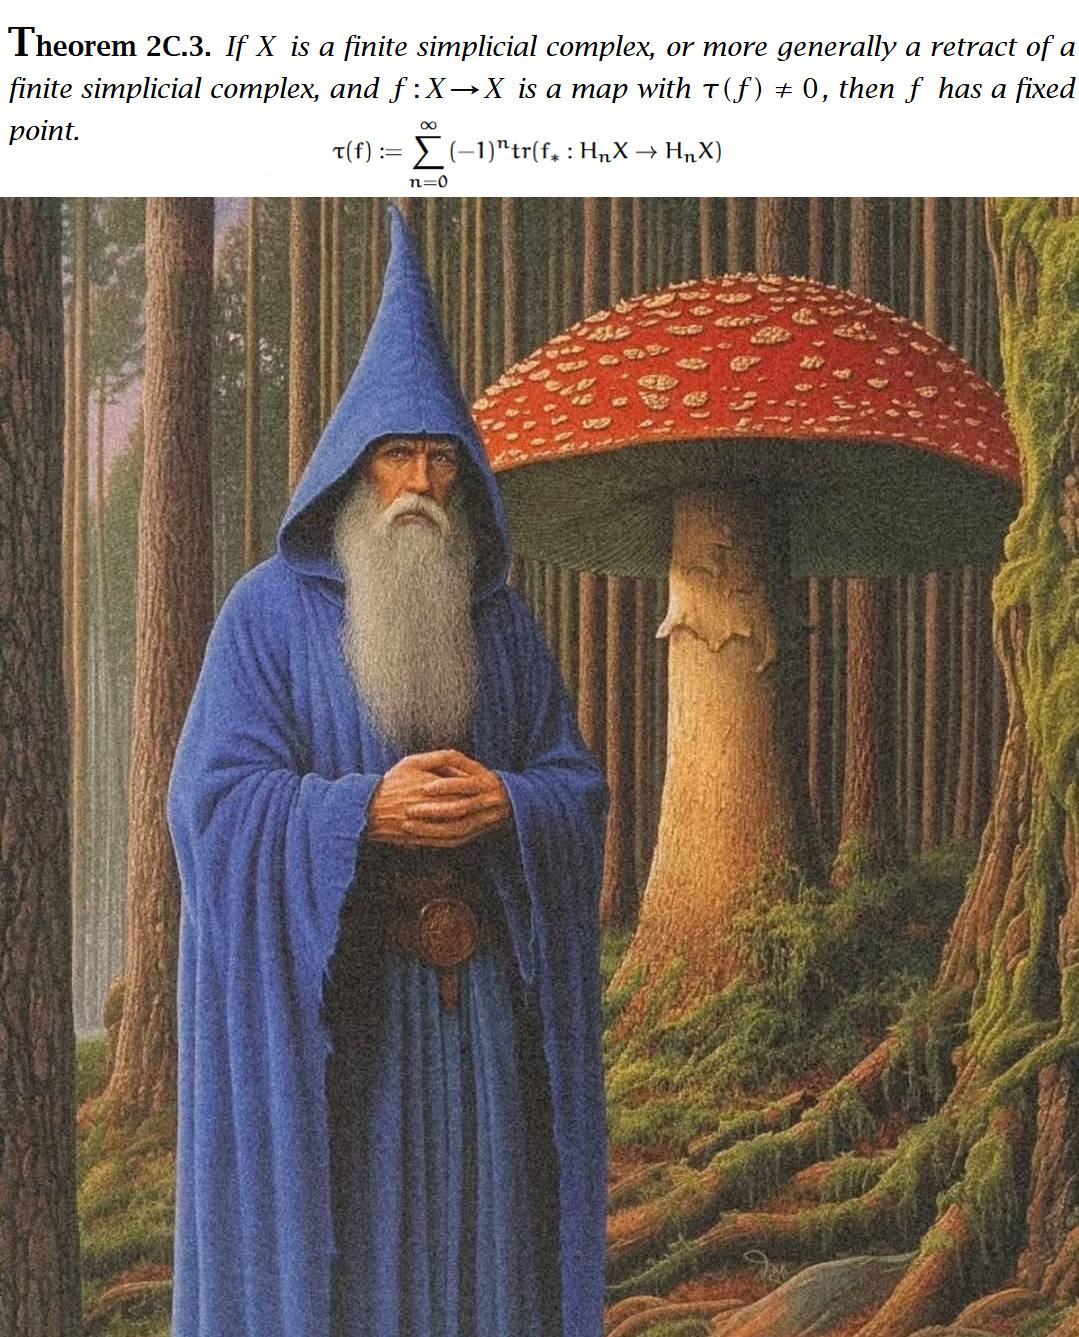
\includegraphics[width=80mm]{lefschetz_number.jpg}
\end{center}

\section{Cohomology}
\subsection{Cohomology Groups}
\subsection{Cup Product}

\begin{center}
    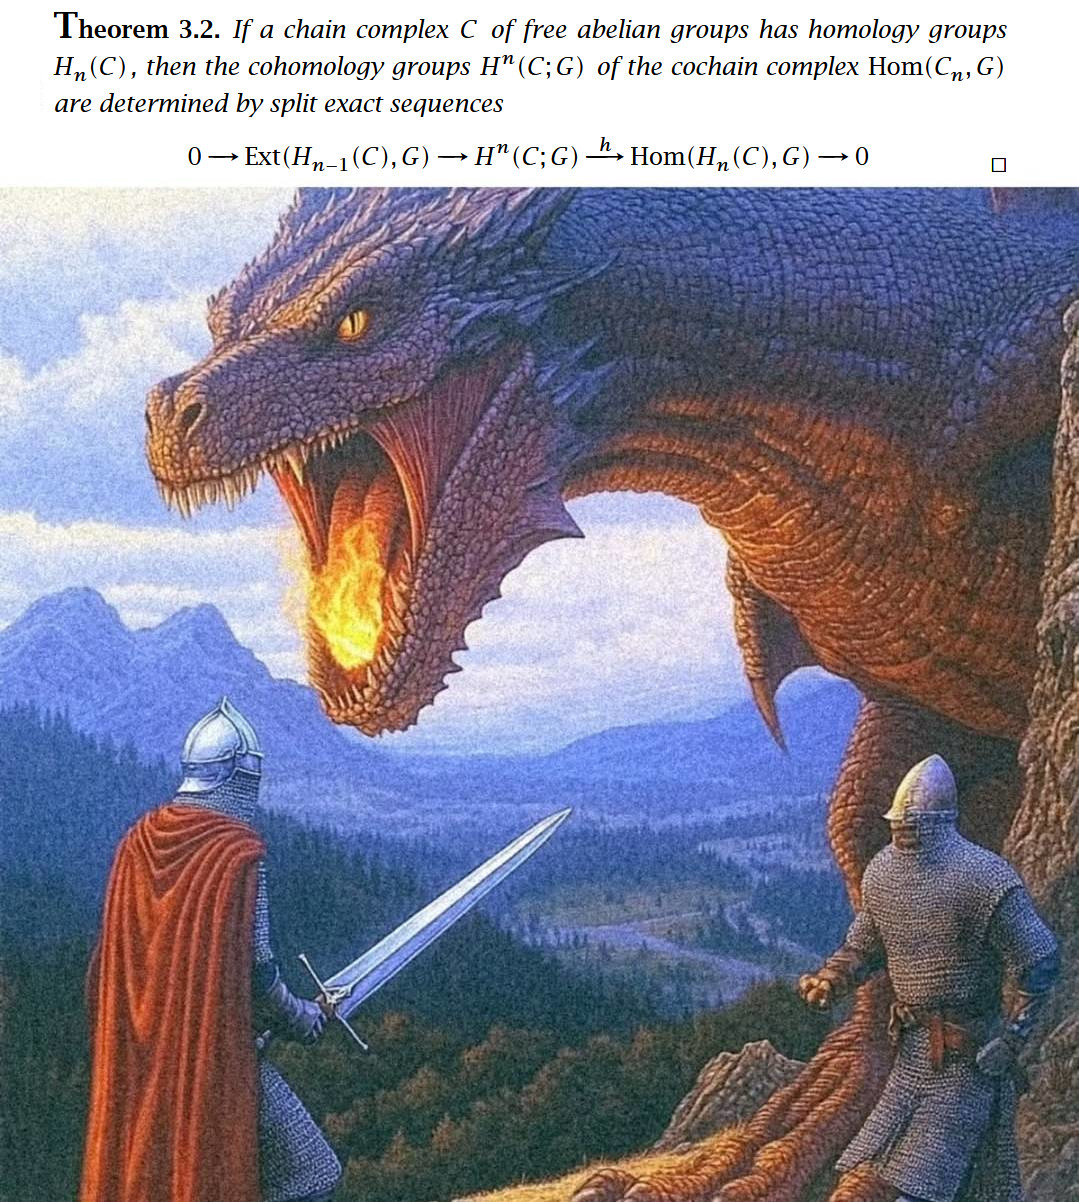
\includegraphics[width=80mm]{cohomology_coefficients.jpg}
\end{center}

\subsection{Poincare Duality}
\subsection{Additional Topics}
\subsubsection{Universal Coefficients for Homology}
\subsubsection{The General K\"unneth Formula}
\subsubsection{$H$-Spaces and Hopf Algebras}
\subsubsection{The Cohomology of $\SO(n)$}
\subsubsection{Bockstein Homomorphisms}
\subsubsection{Limits and $\Ext$}
\subsubsection{Transfer Homomorphisms}
\subsubsection{Local Coefficients}

\printbibliography
\nocite{*}

\clearpage
\thispagestyle{empty}

\begin{center}
    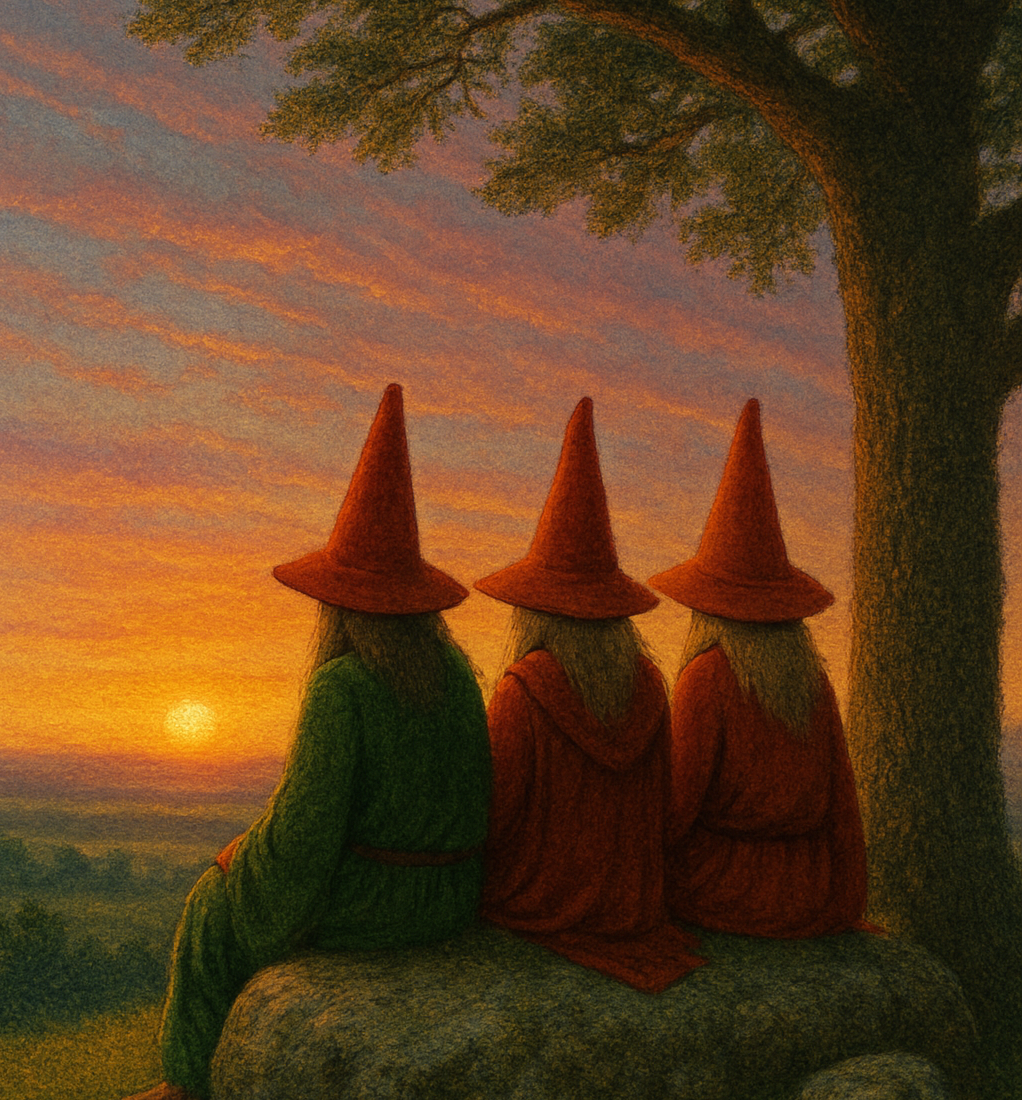
\includegraphics[width=120mm]{happy_ending.png}
\end{center}

\end{document}
